\documentclass[oneside]{book}

\usepackage{ctex}
\usepackage{graphicx}
\usepackage{geometry}
\usepackage[hidelinks]{hyperref}
\usepackage{xcolor}
\hypersetup{
  colorlinks,
  citecolor=violet,
  linkcolor=gray,
  urlcolor=blue}
\geometry{a4paper,scale=0.8}

\title{华东师范大学算法分析助教简易手册}
\author{\href{mailto:zhzhwz@foxmail.com}{zhzhwz@foxmail.com}}

\begin{document}

\frontmatter

\maketitle

\chapter{前言}

\noindent \textbf{简介}

本手册为华东师范大学算法分析课程的助教编写,包含助教工作中可能涉及的各项流程。

\bigbreak

\noindent \textbf{章节介绍}

第 \ref{chap:eoj} 章介绍了 EOJ 的使用方法,着重介绍了 EOJ Polygon 的使用。读者应先阅读前两节,按需阅读第 \ref{sec:polygon_operating_procedures} 节。

第 \ref{chap:elearning} 章介绍了大夏学堂的使用方法。该章暂时无实际内容。

第 \ref{chap:workflow} 章介绍了一些常见的工作流程,读者可在需要完成相应工作时参阅。

\bigbreak

\noindent \textbf{更多}

欢迎在本文的\href{https://github.com/zhzhwz/AlgorithmTAManual}{仓库}提交 issue 或 PR,促进本文的完善。

若遇到无法解决的问题,可在本文的\href{https://github.com/zhzhwz/AlgorithmTAManual}{仓库}提交 issue 或直接\href{mailto:zhzhwz@foxmail.com}{邮件联系作者}。 

若需要其他相关材料(包括各类文档的源文件,各类源代码等),请联系老师或作者。联系作者时请提供简要的身份证明,以避免材料外泄,对教学工作产生影响。

\tableofcontents

\mainmatter

\chapter{EOJ}

\label{chap:eoj}

\section{EOJ 基础}

ECNU Online Judge (EOJ) 是由华东师范大学已毕业的学长开发的在线评测系统。

\subsection{EOJ 的网址}

\href{https://acm.ecnu.edu.cn/}{https://acm.ecnu.edu.cn/}

\subsection{EOJ 的基础用法}

% TODO: add details

请自行摸索或联系作者获取更多信息(我不觉得作者能给你比自行摸索能得到的更多的信息)。

\section{EOJ Polygon 基础}

EOJ Polygon 是 EOJ 的『题目与比赛管理子系统』。

\subsection{如何获取 EOJ Polygon 权限}

\label{ssec:eoj_polygon_permission}

普通用户没有使用 EOJ Polygon 的权限。你需要联系 EOJ 的管理员以获取权限。以下是可能的寻找 EOJ 管理员的方式:

\begin{itemize}
    \item 在 EOJ 主页上寻找管理团队的联系方式(目前为 \href{mailto:acmsupport@admin.ecnu.edu.cn}{acmsupport@admin.ecnu.edu.cn}),联系时表明你的身份和需求(即,需要 EOJ Polygon 的权限),提供你的 EOJ 用户名。(推荐)
    \item 找你的课程老师,让他帮你联系算法竞赛团队的老师要权限
    \item 在 EOJ QQ 群(当前群号:691713742)中问谁是管理员(如果你是社牛可以考虑这个方案)
    \item 联系作者,作者帮你问(不推荐(如果实在不行就来问吧(叹气)))
\end{itemize}

\subsection{使用 EOJ Polygon}

在获取 Polygon 的权限后,你就可以在用户名的下拉菜单(如图 \ref{fig:polygon_entry_user})或者 EOJ 主页的最下方(如图 \ref{fig:polygon_entry_main_page})找到 Polygon 的入口了。EOJ 的主要创建人张羽戈在知乎写了一篇(并没有那么)详尽的文档,包含了几乎所有的 Polygon 的常见用法。详见:\href{https://zhuanlan.zhihu.com/p/59869879}{EOJ Polygon 使用指北 - 知乎}。

\begin{figure}[htbp]
  \centering
  \begin{minipage}{0.28\textwidth}
    \centering
    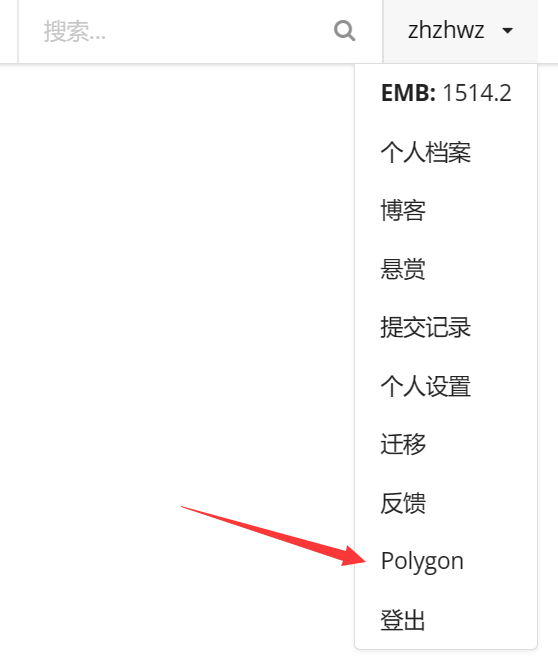
\includegraphics[width=\textwidth]{res/polygon_entry_user.png}
    \caption{用户名下拉菜单处 Polygon 入口}
    \label{fig:polygon_entry_user}
  \end{minipage}
  \begin{minipage}{0.7\textwidth}
    \centering
    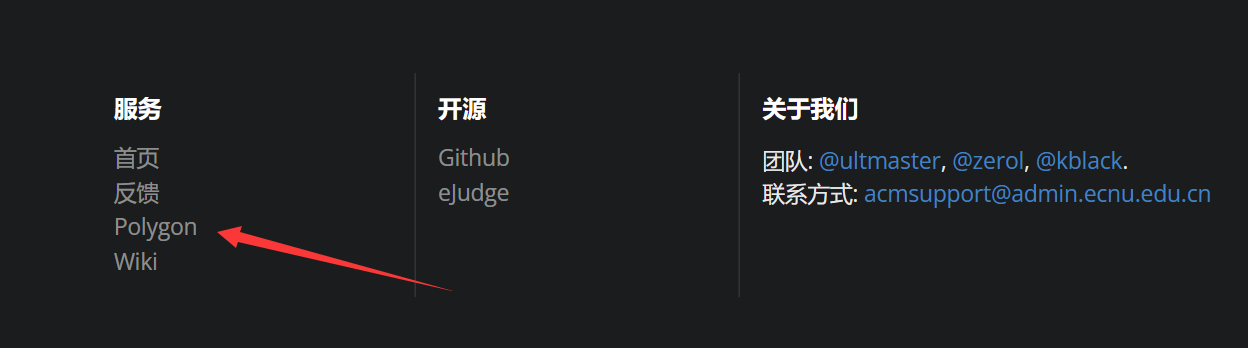
\includegraphics[width=\textwidth]{res/polygon_entry_main_page.png}
    \caption{EOJ 主页最下方处 Polygon 入口}
    \label{fig:polygon_entry_main_page}
  \end{minipage}
\end{figure}

\section{EOJ Polygon 相关常用操作流程}

\label{sec:polygon_operating_procedures}

\subsection{获取往届算法分析作业题和小测题的使用权限}

\label{ssec:permission_get}

以下是可能的方法:

\begin{itemize}
    \item 找你的课程老师,让他给你权限。前提是你的老师拥有对应作业集或比赛的权限。具体的操作步骤为:进入Polygon -- 比赛管理 -- 找到对应的作业集或比赛 -- 进入 -- 修改管理权限 -- 输入并选择要授予权限的用户 -- 点击``必须在这里保存''。
    \item 找作者要权限。前提是作者有权限。
    \item 如果想要其他作业集的权限,联系对应作业集或比赛的管理员,或直接联系 EOJ 的管理员(联系方法参见第 \ref{ssec:eoj_polygon_permission} 小小节)。
\end{itemize}

\textbf{\textcolor{red}{注意:请务必在你创建的作业集或比赛中,在管理权限中加上你的老师。否则以后的助教就只能来找你要权限了。(你也可以在管理权限中加上作者(EOJ 用户名:zhzhwz))}}

\subsection{创建一个作业集或比赛}

\label{ssec:create_homework_set}

\subsection{导入学生名单}

\label{ssec:import_student_list}

\subsection{导出邀请码}

\label{ssec:export_inviting_code}

\subsection{复制现有的题目}

\label{ssec:copy_exist_problem}

\subsection{创建题目}

\label{ssec:create_new}

\subsection{将题目添加到作业集或比赛}

\label{ssec:add_problem_to_homework_set}

\subsection{更新题目}

\label{ssec:update_problem}

\subsection{重判题目}

\label{ssec:rejudge_problem}

\chapter{大夏学堂}

\label{chap:elearning}

% TODO: add details

大夏学堂有什么能讲的呢?自己摸索或者看大夏学堂的文档去吧。(主要是作者现在也登不进大夏学堂了)(欢迎补充该部分文档)

\chapter{常见工作流程}

\label{chap:workflow}

\section{创建作业集}

% TODO: finish it

\section{布置一次作业}

\begin{enumerate}
  \item 和老师沟通,确定本次作业的题数和每题的主题或涉及算法。
  \item 寻找相关题目。以下是可能的方法:
  \begin{itemize}
    \item 在之前的作业集中选择合适的题目。若无对应作业集权限,参考第 \ref{ssec:permission_get} 小小节的方法获得之前作业集的权限。
    \item 在 EOJ 公开题目中寻找相关题目。
    \item 在其他 OJ 获取题面和数据。作者已知目前唯一能够方便获取数据的 OJ 仅有 \href{https://loj.ac/}{LOJ} ,但其题目难度普遍偏高,请谨慎挑选。
    \item 在其他 OJ 获得题面,并自己造数据。包括但不限于\href{https://www.luogu.com.cn/}{洛谷}等 OJ 的题面可以直接在题目界面复制 markdown 源代码。造数据的方法可以参见第 \ref{sec:generating_data} 节。
    \item 从零开始自行创建题目。见第 \ref{chap:create_problem} 章。
  \end{itemize}
  \item 和老师沟通选定的题目是否合适。
  \item 复制现有的题目,见第 \ref{ssec:copy_exist_problem} 小节;或创建题目,见第 \ref{ssec:create_new} 小节。
  \item 将题目添加到作业集,见第 \ref{ssec:create_homework_set} 小节。
\end{enumerate}

\section{准备一次小测}

% TODO: finish it

\chapter{从零开始创建一道题}

\label{chap:create_problem}

本章的内容对于无算法竞赛基础的读者可能难度较大。考虑到实际工作中可能会用到,此处给出一些简单的指引。若读完仍感觉无从下手,请咨询身边的朋友(如,有算法竞赛经历或出题经历的同学等)。

除了本文外,你也可以参考一些网络上的资料,如\href{https://oi-wiki.org/contest/problemsetting/}{出题 - OI-Wiki}等。

% TODO: finish it

\section{编写题面}

\section{编写标程}

\section{造数据}

\label{sec:generating_data}

\section{测试部分分}

\section{验题}

\end{document}
